\hypertarget{_nessie_exception_8hpp}{
\subsection{NessieException.hpp File Reference}
\label{_nessie_exception_8hpp}\index{NessieException.hpp(175)@{NessieException.hpp(175)}}
}
Declaration of \hyperlink{class_nessie_exception}{NessieException} class.  


{\tt \#include $<$string$>$}\par
{\tt \#include $<$exception$>$}\par


Include dependency graph for NessieException.hpp:\nopagebreak
\begin{figure}[H]
\begin{center}
\leavevmode
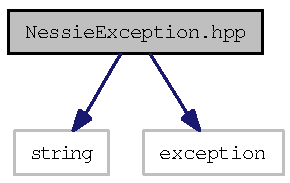
\includegraphics[width=87pt]{_nessie_exception_8hpp__incl}
\end{center}
\end{figure}


This graph shows which files directly or indirectly include this file:\nopagebreak
\begin{figure}[H]
\begin{center}
\leavevmode
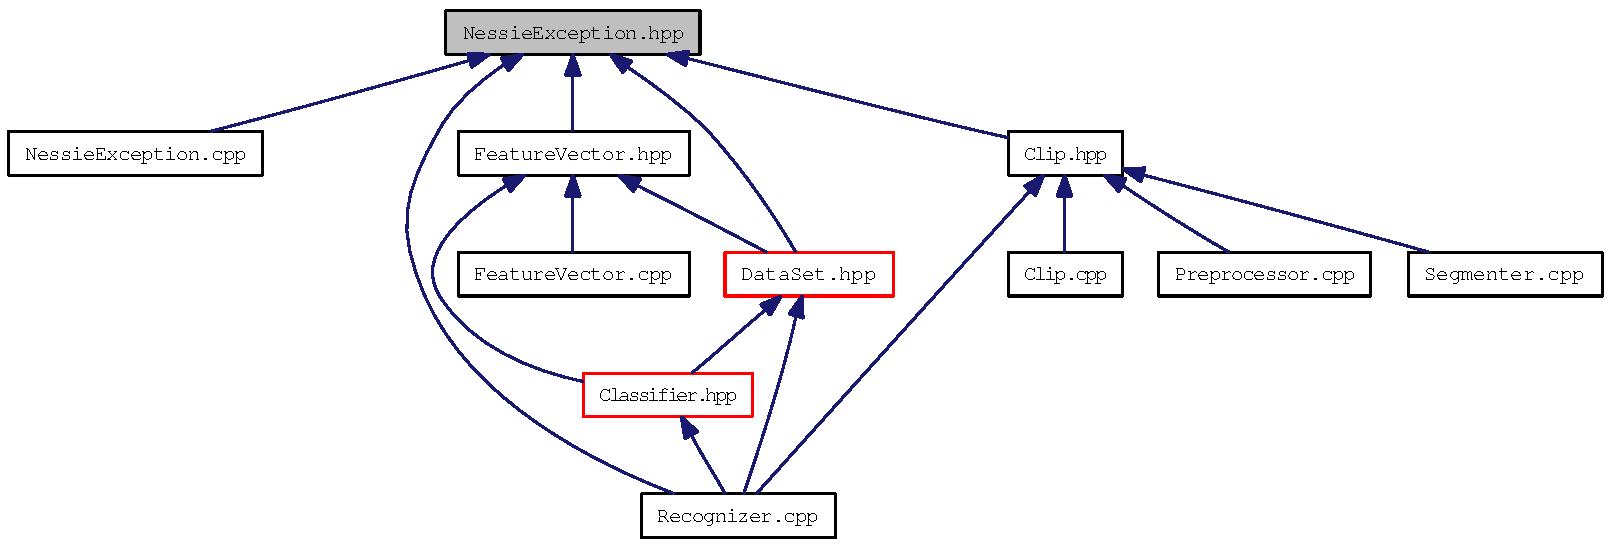
\includegraphics[width=270pt]{_nessie_exception_8hpp__dep__incl}
\end{center}
\end{figure}
\subsubsection*{Data Structures}
\begin{CompactItemize}
\item 
class \hyperlink{class_nessie_exception}{NessieException}
\begin{CompactList}\small\item\em Exception raised by a Nessie OCR object. \item\end{CompactList}\end{CompactItemize}


\subsubsection{Detailed Description}
Declaration of \hyperlink{class_nessie_exception}{NessieException} class. 

